\documentclass[tikz]{standalone}
\usepackage{tikz}
\usepackage{fourier-otf}
\usepackage{fontspec}

\begin{document}
	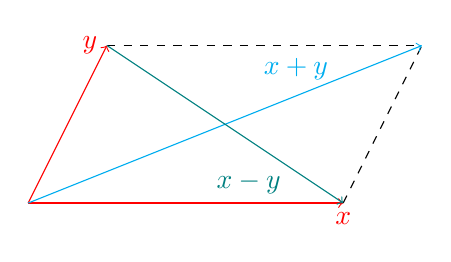
\begin{tikzpicture}
		\coordinate (O) at (0, 0);
		\coordinate (X) at (4, 0);
		\coordinate (Y) at (1, 2);
		\coordinate (A) at (5, 2);
		
		\draw[->, color=red] (O) -- (X) node[below]{$x$};
		\draw[->, color=red] (O) -- (Y) node[left]{$y$};
		\draw[dashed] (X) -- (A);
		\draw[dashed] (Y) -- (A);
		\draw[->, color=cyan] (O) -- (A) node[shift={(-1.6,-0.3)}]{$x+y$};
		\draw[->, color=teal] (Y) -- (X) node[shift={(-1.2,0.25)}]{$x-y$};
	\end{tikzpicture}
\end{document}